\documentclass[12pt,a4paper]{article}
\usepackage[utf8]{inputenc} % sempre salve seus arquivos como UTF8
\usepackage[T1]{fontenc}
\usepackage[english]{babel}

\usepackage[left=2.5cm,right=2cm,top=2cm,bottom=2.5cm]{geometry}
\usepackage{amsmath}
\usepackage{amsthm}
\usepackage{amsfonts}

\usepackage{graphicx}
\usepackage{algorithm}
\usepackage{color}
\usepackage[noend]{algpseudocode}
\usepackage{mathtools}
\usepackage{subfig}
\usepackage{diagbox}

% load times font
\usepackage{mathptmx}
\usepackage[scaled=.90]{helvet}
\usepackage{courier}

% comandos
\newcommand{\mdc}[1]{\mathrm{mdc}(#1)}

\DeclarePairedDelimiter\ceil{\lceil}{\rceil}
\DeclarePairedDelimiter\floor{\lfloor}{\rfloor}

% Foot without marker
\newcommand\blfootnote[1]{%
	\begingroup
	\renewcommand\thefootnote{}\footnote{#1}%
	\addtocounter{footnote}{-1}%
	\endgroup
}

\title{MO446 -- Introduction to Computer Vision  \\ Project 1}
\author{Breno Leite  \\ Guilherme Leite}
\date{28/08/2017}

\begin{document}

\maketitle
\blfootnote{\textit{\textbf{Important note:} The borders seen in the figures are not part of the image, they are figurative information about the starting and ending points of the image. Moreover, all the image scales in this report were changed in order to make the text more readable.}} \\

%% ---------------- Starts here --------------------------------

\textbf{\LARGE Input Images}\\

Throughout this project some images are used as input to test the algorithms. Figure \ref{fig:p1-1-0} was used as input for the pyramids exercises \textbf{2.1, 2.2, 2.3} and \textbf{3.1}, its dimensions are 400x300 and it is a colored image. \\

\begin{figure}[!h]
	\centering
	{%
		\setlength{\fboxsep}{1pt}%
		\setlength{\fboxrule}{1pt}%
		\fbox{
\includegraphics[scale=1]{input/p1-1-0}}%
	}%
	\caption{Input image for pyramids and Fourier transform exercises. (\textbf{p1-1-0})}
	\label{fig:p1-1-0}
\end{figure}

\newpage

Images in Figure \ref{fig:blending} are used for the blending exercises (\textbf{2.4} and \textbf{3.2}), their dimensions is 540x392. Note that the images are slightly rotated, this will affect some results which comes from the image and not by any error on the process itself.\\

\begin{figure}[!h]
	\centering
	\subfloat[An arbitrary orange (\textbf{p1-2-4-0})]{
		{
			\setlength{\fboxsep}{1pt}
			\setlength{\fboxrule}{1pt}
			\fbox{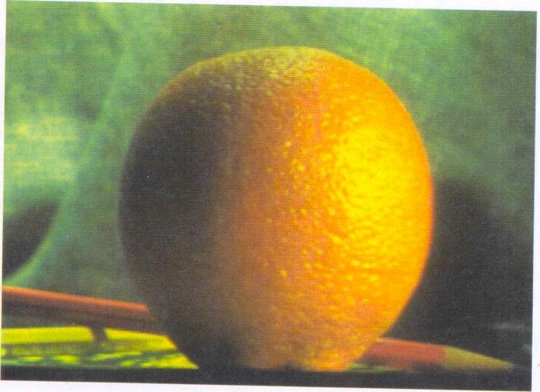
\includegraphics[scale=0.5]{input/p1-2-4-0}}
		}
	}
	\quad
	\subfloat[An arbitrary apple (\textbf{p1-2-4-1})]{
		{
			\setlength{\fboxsep}{1pt}
			\setlength{\fboxrule}{1pt}
			\fbox{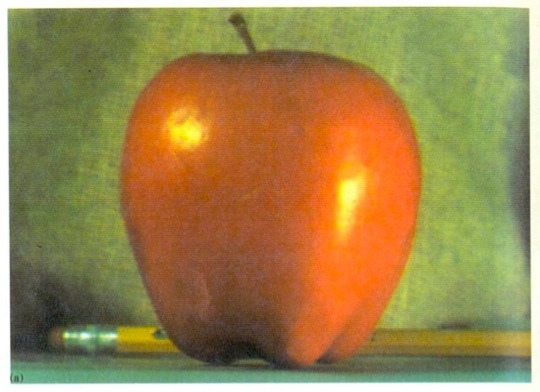
\includegraphics[scale=0.5]{input/p1-2-4-1}}
		}
	}
	\quad
	\subfloat[Mask for blending (\textbf{p1-2-4-2})]{
		{
			\setlength{\fboxsep}{1pt}
			\setlength{\fboxrule}{1pt}
			\fbox{
\includegraphics[scale=0.25]{input/p1-2-4-2}}
		}
	}
	\caption{Images used on the blending experiments.}
	\label{fig:blending}
\end{figure}
	
\textbf{\LARGE Question 2 - Spatial blending}\\

\textbf{2.1 )} Convolution can be understood as the action of applying a kernel to an image, in this case every pixel in the image is affected by the weighted sum of the filter applied to the pixel neighborhood. This approach requires some special attention when dealing with the edges of the image, since the application of the kernel will overshoot the image borders. Our solution to this problem was to extend the original image filling its new borders with zeros. \\

A minor downside of this approach is the lessen effect of the kernel around the edges, this solution was chosen for its simplicity to implement. Additionally, the convolution was tested with three different Gaussians smoothing kernels, with sizes 3x3, 7x7 and 15x15. In comparison to the embedded solution by OpenCV our convolution was noticeably slower as seen in Table \ref{table:convolution-opencv}. Our intuition about this is that the OpenCV is running C code, which is highly optimized. \\ 

\begin{table}[!h]
	\centering
	\begin{tabular}{|c|c|c|c|}
		\hline
		& \multicolumn{3}{c|}{\textbf{Time (seconds)}} \\ \hline
		\backslashbox{\textbf{Convolution}}{\textbf{Kernel Size}}    & \textbf{3x3}         & \textbf{7x7}          & \textbf{15x15}      \\ \hline
		\textbf{Implemented}  & 4.481      & 4.535      & 5.083     \\ \hline
		\textbf{OpenCV} & 0.001      & 0.004       & 0.010     \\ \hline
	\end{tabular}
	\caption{Comparison between our implementation and OpenCV convolution time.}
	\label{table:convolution-opencv}
\end{table}

As expected the kernel smooth the edges around the image and suffers with a darkening close to the borders as seeing in Figure \ref{fig:p1-2-1-0}, with bigger kernel the image suffered more distortion to the point of loosing all of its fine details (Figure \ref{fig:p1-2-1-2}). The loss of these details is accounted by the size of the neighborhood that affected each pixel, thus a larger kernel smooths more than a smaller one. \\

\begin{figure}[!h]
	\centering
	\subfloat[3x3 Kernel (\textbf{p1-2-1-0})]{
		{
			\setlength{\fboxsep}{1pt}
			\setlength{\fboxrule}{1pt}
			\fbox{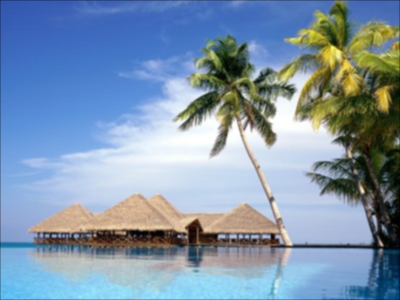
\includegraphics[scale=0.3]{output/p1-2-1-0}}
		}
		\label{fig:p1-2-1-0}
	}
	\quad
	\subfloat[7x7 Kernel (\textbf{p1-2-1-1})]{
		{
			\setlength{\fboxsep}{1pt}
			\setlength{\fboxrule}{1pt}
			\fbox{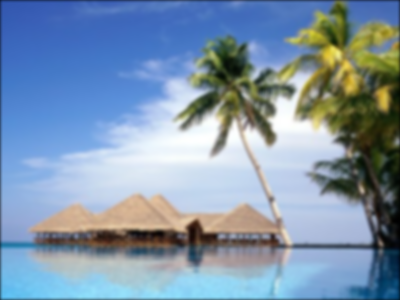
\includegraphics[scale=0.3]{output/p1-2-1-1}}
		}
	}
	\quad
	\subfloat[15x15 Kernel (\textbf{p1-2-1-2})]{
		{
			\setlength{\fboxsep}{1pt}
			\setlength{\fboxrule}{1pt}
			\fbox{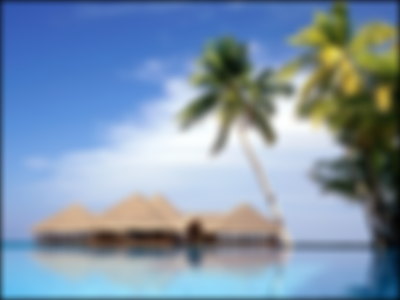
\includegraphics[scale=0.3]{output/p1-2-1-2}}
		}
		\label{fig:p1-2-1-2}
	}
	\caption{Convolution results applying different Gaussian kernels.}
	\label{fig:convolution}
\end{figure}

\textbf{2.2 )} To store the Gaussian and Laplacian pyramids on this project we used a linked list, in which each node holds a level of the pyramid. Since the data structure is a list the access method is as in a array, e.g. $pyramid[i]$ returns the image in the ith pyramid level, disregarding the necessity to implement an access function. \\

The strategy chosen to implement the interpolation was the bilinear interpolation. These decisions were taken regarding the time to implement and simplicity to understand. It is also worth noting that due to some confusion about the meaning of Up and Down, these functions were renamed as follow: Expand referring to the action of expand the image width and height, and Contract analogously. Figure \ref{fig:gaussianPyramid} shows the pyramid formed with the implemented function. \\

\begin{figure}[!h]
	\centering
	\subfloat[3rd level (\textbf{p1-2-2-0})]{
		{
			\setlength{\fboxsep}{1pt}
			\setlength{\fboxrule}{1pt}
			\fbox{
\includegraphics[scale=0.5]{output/p1-2-2-0}}
		}
	}
	\quad
	\subfloat[2nd level (\textbf{p1-2-2-1})]{
		{
			\setlength{\fboxsep}{1pt}
			\setlength{\fboxrule}{1pt}
			\fbox{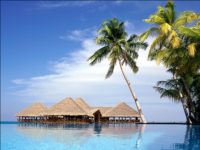
\includegraphics[scale=0.5]{output/p1-2-2-1}}
		}
	}
	\quad
	\subfloat[1st level (\textbf{p1-2-2-2})]{
		{
			\setlength{\fboxsep}{1pt}
			\setlength{\fboxrule}{1pt}
			\fbox{
\includegraphics[scale=0.5]{output/p1-2-2-2}}
		}
	}
	\caption{Images composing the levels on the Gaussian Pyramid formed from image \textbf{p1-1-0}}
	\label{fig:gaussianPyramid}
\end{figure}

\textbf{2.3 )} The Laplacian pyramid demanded more attention to its details, like the fact that the last level of the pyramid is a copy of the same level at the Gaussian pyramid. This particular level is used to perform the reconstruction of the original image, first the image is extended and interpolated to match the previous level size. And then, it is summed with the previous level of the pyramid. The repetition of these steps result on the original image that was compressed in the pyramid, Figure \ref{fig:placePyramid} shows the Laplacian pyramid. \\

\begin{figure}[!h]
	\centering
	\subfloat[(\textbf{p1-2-3-0})]{
		{
			\setlength{\fboxsep}{1pt}
			\setlength{\fboxrule}{1pt}
			\fbox{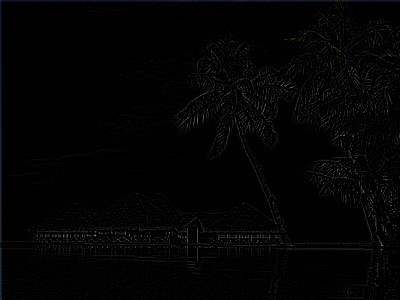
\includegraphics[scale=0.5]{output/p1-2-3-0}}
		}
	}
	\quad
	\subfloat[(\textbf{p1-2-3-1})]{
		{
			\setlength{\fboxsep}{1pt}
			\setlength{\fboxrule}{1pt}
			\fbox{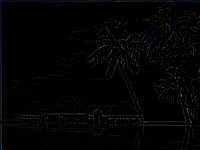
\includegraphics[scale=0.5]{output/p1-2-3-1}}
		}
	}
	\quad
	\subfloat[(\textbf{p1-2-3-2})]{
		{
			\setlength{\fboxsep}{1pt}
			\setlength{\fboxrule}{1pt}
			\fbox{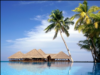
\includegraphics[scale=0.5]{output/p1-2-3-2}}
		}
	}
	\caption{Images (a), (b) and (c) composing the levels on Laplacian Pyramid formed from image \textbf{p1-1-0}}
	\label{fig:placePyramid}
\end{figure}


\textbf{2.4 )} The process of blending two images implemented here is referred as "Splining Regions of Arbitrary Shape" in Burt and Adelson's paper, it consists of three gaussian pyramids $GA$, $GB$ and $GM$, and three laplacian pyramids $LA$, $LB$ and $LS$, in which $LS$ is the resulting pyramid and the image at its base is the blended image. The algorithm to blend the images uses both $LA$, $LB$ and $GM$ pyramids simultaneously, from their top it multiply each lower resolution image with the equivalent mask (Figure \ref{fig:blendingProcess} (a) and (b)), sum the resulting images with each other (Figure \ref{fig:blendingProcess} (c)) and expand the resulting image, repeat these steps and the resulting image at the base of $LS$ is the blended image. The core point of this process is the gaussian filter applied to the mask that smooth its borders and the expand operation performed in the pyramid. Two tests were performed reproducing the original results, in Figure \ref{fig:blending} (a) and (b) were merged using Figure \ref{fig:blending} (c) as mask and Figure \ref{fig:blendingFurther} (a) and (b) were merged using Figure \ref{fig:blendingFurther} (c) as mask, resulting in Figure \ref{fig:blendingResult} (b).

\begin{figure}[!h]
	\centering
	\subfloat[Mask p1-2-4-2 multiplied with image p1-2-4-0 (\textbf{report-p1-2-4-0})]{
		{
			\setlength{\fboxsep}{1pt}
			\setlength{\fboxrule}{1pt}
			\fbox{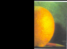
\includegraphics[scale=1.5]{report/p1-2-4-0}}
		}
	}
	\quad
	\subfloat[Inverted mask p1-2-4-2 multiplied with image p1-2-4-1 (\textbf{report-p1-2-4-1})]{
		{
			\setlength{\fboxsep}{1pt}
			\setlength{\fboxrule}{1pt}
			\fbox{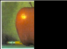
\includegraphics[scale=1.5]{report/p1-2-4-1}}
		}
	}
	\quad
	\subfloat[Sum of both (a) with (b) (\textbf{report-p1-2-4-2})]{
		{
			\setlength{\fboxsep}{1pt}
			\setlength{\fboxrule}{1pt}
			\fbox{
\includegraphics[scale=1.5]{report/p1-2-4-2}}
		}
	}
	\caption{Images (a) and (b) are the result of the blending operation.}
	\label{fig:blendingProcess}
\end{figure}

\begin{figure}[!h]
	\centering
	\subfloat[(\textbf{p1-2-4-3})]{
		{
			\setlength{\fboxsep}{1pt}
			\setlength{\fboxrule}{1pt}
			\fbox{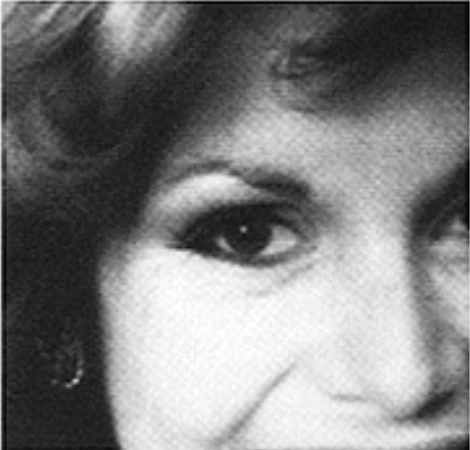
\includegraphics[scale=0.25]{input/p1-2-4-3}}
		}
	}
	\quad
	\subfloat[(\textbf{p1-2-4-4})]{
		{
			\setlength{\fboxsep}{1pt}
			\setlength{\fboxrule}{1pt}
			\fbox{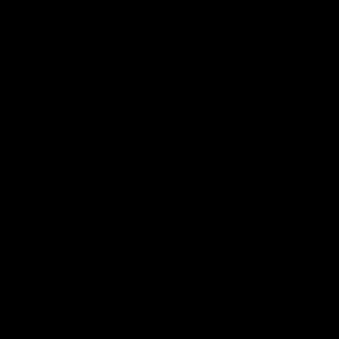
\includegraphics[scale=0.25]{input/p1-2-4-4}}
		}
	}
	\quad
	\subfloat[(\textbf{p1-2-4-5})]{
		{
			\setlength{\fboxsep}{1pt}
			\setlength{\fboxrule}{1pt}
			\fbox{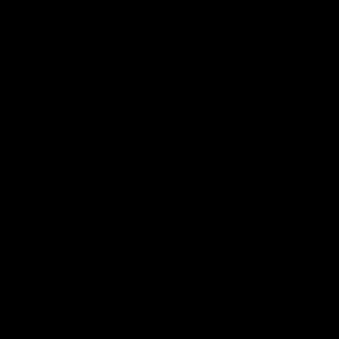
\includegraphics[scale=0.25]{input/p1-2-4-5}}
		}
	}
	\caption{Images (a), (b) and (c) used for further testing the blending operations.}
	\label{fig:blendingFurther}
\end{figure}

\begin{figure}[!h]
	\centering
	\subfloat[(\textbf{p1-2-4-0})]{
		{
			\setlength{\fboxsep}{1pt}
			\setlength{\fboxrule}{1pt}
			\fbox{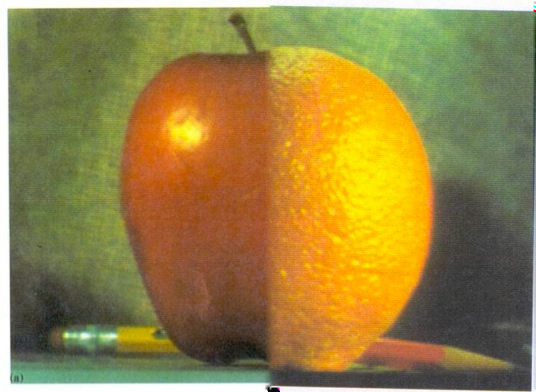
\includegraphics[scale=0.25]{output/p1-2-4-0}}
		}
	}
	\quad
	\subfloat[(\textbf{p1-2-4-1})]{
		{
			\setlength{\fboxsep}{1pt}
			\setlength{\fboxrule}{1pt}
			\fbox{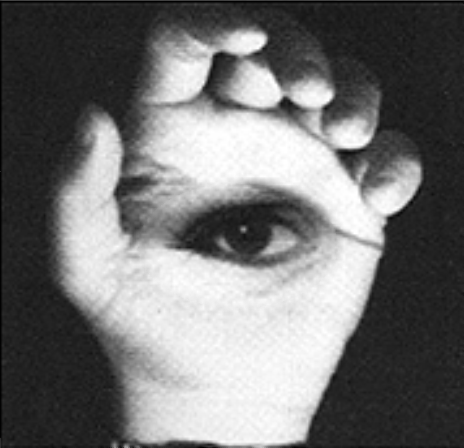
\includegraphics[scale=0.25]{output/p1-2-4-1}}
		}
	}
	\caption{Images (a) and (b) are the result of the blending operation.}
	\label{fig:blendingResult}
\end{figure}

\newpage

\textbf{\LARGE Question 3 - Frequency Blending} \\

In this question, we will present some experiments developed using \emph{numpy} and \emph{OpenCV} functions in order to transform the image from spatial domain to frequency domain. The process will be divided into two different experiments for better readability. \\

On the first one (\textbf{3.1}), we will be modifying the phase and magnitude in order to see the impact on the image recontructed on the Fourier transform. On the second experiment (\textbf{3.2}), we will be blending the two images used in Question \textbf{4.2} in order to compare frequency and spatial blending. \\

\textbf{3.1 )} Exploring Fourier Space \\

To explore the Fourier space, we implemented two functions different functions. The first one is responsible to transform an image into vectors of magnitude and phase, while the other is responsible to reconstruct the image from the magnitude and phase vectors. The Figure \ref{fig:mag-phase} shows the magnitude and phase obtained transforming the Figure \ref{fig:p1-1-0} to the frequency domain. \\

\begin{figure}[!h]
	\centering
	\subfloat[Phase Image (\textbf{p1-3-1-0})]{
		{
			\setlength{\fboxsep}{1pt}
			\setlength{\fboxrule}{1pt}
			\fbox{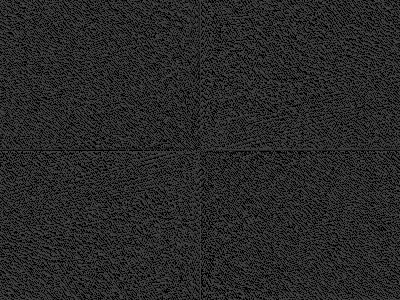
\includegraphics[scale=0.5]{output/p1-3-1-0}}
		}
		\label{fig:phase}
	}
	\quad
	\subfloat[Magnitude Image (\textbf{p1-3-1-1})]{
		{
			\setlength{\fboxsep}{1pt}
			\setlength{\fboxrule}{1pt}
			\fbox{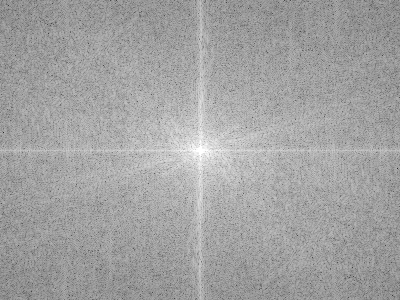
\includegraphics[scale=0.5]{output/p1-3-1-1}}
		}
		\label{fig:magnitude}
	}
	\caption{Images representing phase and magnitude on the Fourier transform using image \textbf{p0-1-0}.}
	\label{fig:mag-phase}
\end{figure}

In order to represent these images, the results from the Fourier transform were shifted to the center and also reduced by the functions, $20*log_e(magnitude)$ and $40*log_e(phase)$, in which $magnitude$ and $phase$ are vectors from the transformation. The reduction is necessary to keep the numbers in a range from 0 to 255, which is showed into the image. This normalization does not affect the transformation, the values are converted back on before the reverse Fourier transform. \\

The Figure \ref{fig:phase} represents the phase, it is quite hard to obtain any information from this representation. Moreover, the Figure \ref{fig:magnitude} represents the magnitude of the image, brightness on the magnitude image represents high frequencies on the original image. In this way, the magnitude indicates that image \textbf{p1-1-0} has more high than low frequencies, the intuition comes from the high brightness on the magnitude image. \\

In the next experiments, we will be modifying the values of the phase and magnitude before the reverse Fourier transform, this process should reconstruct the original image when using the same phase and image. In order to modify the magnitude, we used a percentage of the pixels from the magnitude or phase, the rest of the pixels were zeroed out. In the experiment this process uses only 1 pixel, 25\%, 50\%, 75\% and 100\% of the pixels. \\

This pixels used might be in two different ways, highest or lowest, e.g. 25\% lowest pixels on phase image would maintain the values and the rest would be zeroed out. As expected, all the images reconstruct using 100\% of the pixels in magnitude and phase were perfectly reconstruct (Figure \ref{fig:inverse}). The following experiments were made using the Figure \ref{fig:p1-1-0} in grayscale, the grayscale was used for more simplicity and further on one experiment will show the same results in a colored image to prove algorithm capacities. \\


\begin{figure}[!h]
	\centering
	{%
		\setlength{\fboxsep}{1pt}%
		\setlength{\fboxrule}{1pt}%
		\fbox{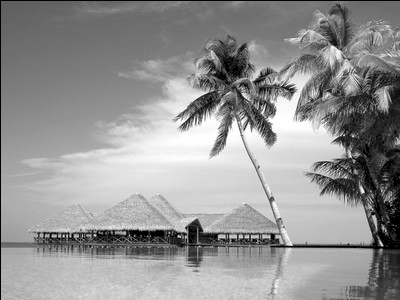
\includegraphics[scale=0.55]{output/p1-3-1-6}}%
	}%
	\caption{Reconstructed image from inverse Fourier transform using 100\% of pixels in magnitude and phase. (\textbf{p1-3-1-6, p1-3-1-11, p1-3-1-16, and p1-3-1-21})}
	\label{fig:inverse}
\end{figure}


In order to show the differences when modifying the phase or magnitude image, we will divide the experiments into two parts, also for better readability. \\

\begin{itemize}
	\item \textbf{Phase} - First we will be modifying the phase image and performing the inverse Fourier transform. In this experiment we were expecting changes on the position of the objects. The Figure \ref{fig:phaseINC} show the results when using the lowest values of the phase image. \\

	\begin{figure}[!h]
		\centering
		\subfloat[Only lowest pixel (\textbf{p1-3-1-2})]{
			{
				\setlength{\fboxsep}{1pt}
				\setlength{\fboxrule}{1pt}
				\fbox{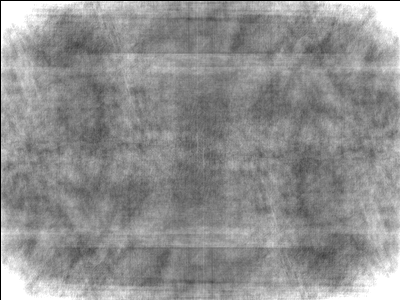
\includegraphics[scale=0.4]{output/p1-3-1-2}}
			}
			\label{fig:phaseinc1}
		}
		\quad
		\subfloat[Lowest 25\% pixels (\textbf{p1-3-1-3})]{
			{
				\setlength{\fboxsep}{1pt}
				\setlength{\fboxrule}{1pt}
				\fbox{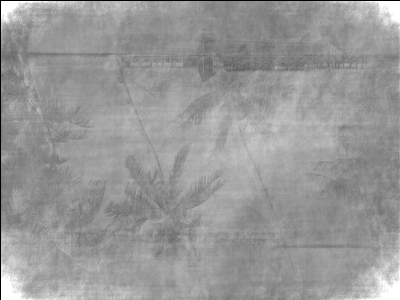
\includegraphics[scale=0.4]{output/p1-3-1-3}}
			}
			\label{fig:phaseinc25}
		}
		\quad
		\subfloat[Lowest 50\% pixels (\textbf{p1-3-1-4})]{
			{
				\setlength{\fboxsep}{1pt}
				\setlength{\fboxrule}{1pt}
				\fbox{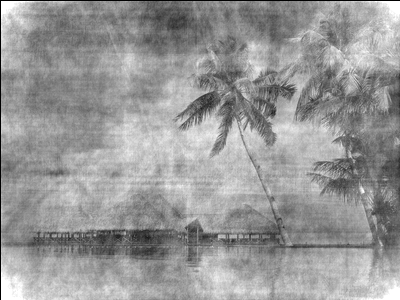
\includegraphics[scale=0.4]{output/p1-3-1-4}}
			}
			\label{fig:phaseinc50}
		}
		\quad
		\subfloat[Lowest 75\% pixels (\textbf{p1-3-1-5})]{
			{
				\setlength{\fboxsep}{1pt}
				\setlength{\fboxrule}{1pt}
				\fbox{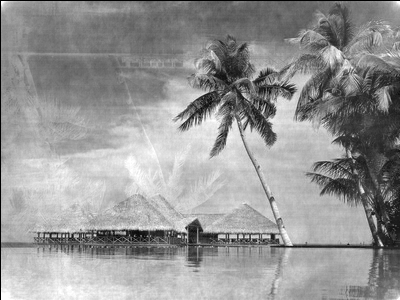
\includegraphics[scale=0.4]{output/p1-3-1-5}}
			}
			\label{fig:phaseinc75}
		}
		
		\caption{Results obtained by inverse Fourier transform using lowest pixels on phase image.}
		\label{fig:phaseINC}
	\end{figure}
	
	As we can see the image shows us information about orientations, in this way, selecting different values changes the orientation of the image. Another interesting fact is the upside down elements on the reconstructed images, our intuition is that it happen because of the range in which the transform is working (0 to 380 degrees). In other hand, the Figure \ref{fig:phaseDESC} shows the results on the reverse transform using the highest pixels on phase image. \\
	
	\begin{figure}[!h]
		\centering
		\subfloat[Only highest pixel (\textbf{p1-3-1-7})]{
			{
				\setlength{\fboxsep}{1pt}
				\setlength{\fboxrule}{1pt}
				\fbox{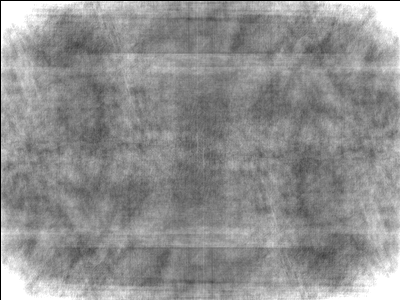
\includegraphics[scale=0.4]{output/p1-3-1-7}}
			}
			\label{fig:phasedesc1}
		}
		\quad
		\subfloat[Highest 25\% pixels (\textbf{p1-3-1-8})]{
			{
				\setlength{\fboxsep}{1pt}
				\setlength{\fboxrule}{1pt}
				\fbox{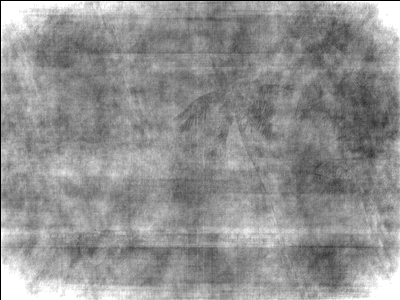
\includegraphics[scale=0.4]{output/p1-3-1-8}}
			}
			\label{fig:phasedesc25}
		}
		\quad
		\subfloat[Highest 50\% pixels (\textbf{p1-3-1-9})]{
			{
				\setlength{\fboxsep}{1pt}
				\setlength{\fboxrule}{1pt}
				\fbox{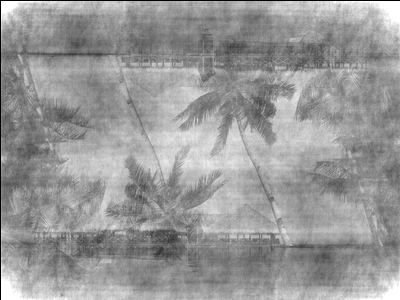
\includegraphics[scale=0.4]{output/p1-3-1-9}}
			}
			\label{fig:phasedesc50}
		}
		\quad
		\subfloat[Highest 75\% pixels (\textbf{p1-3-1-10})]{
			{
				\setlength{\fboxsep}{1pt}
				\setlength{\fboxrule}{1pt}
				\fbox{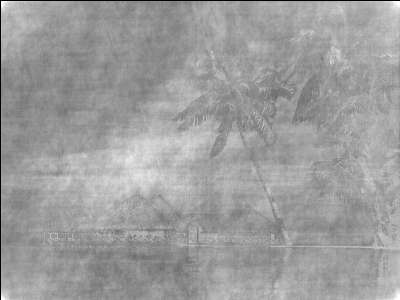
\includegraphics[scale=0.4]{output/p1-3-1-10}}
			}
			\label{fig:phasedesc75}
		}
		
		\caption{Results obtained by inverse Fourier transform using highest pixels on phase image.}
		\label{fig:phaseDESC}
	\end{figure}
	
	An interesting feature is that the images contain complement information, as example the Figure \ref{fig:phasedesc25} has less information than Figure \ref{fig:phaseinc75} about the original image, however their information is complementary. The same effect might be seen in the other images as well. \\
	
	\item \textbf{Magnitude} -  In this part we will be doing similar experiments, but this time, modifying the magnitude image. In addition, we expect to see different results on the intensity on the reconstructed images, which is described by the magnitude on the frequency domain. The Figure \ref{fig:magnitude} shows the different images obtained on the inverse Fourier transform. \\
	
	\begin{figure}[!h]
		\centering
		\subfloat[Only lowest pixel (\textbf{p1-3-1-12})]{
			{
				\setlength{\fboxsep}{1pt}
				\setlength{\fboxrule}{1pt}
				\fbox{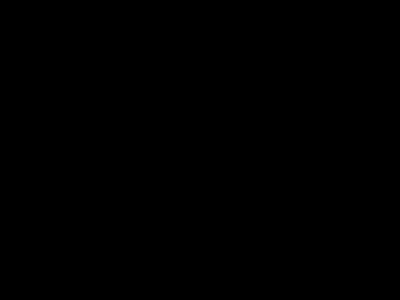
\includegraphics[scale=0.3]{output/p1-3-1-12}}
			}
			\label{fig:magnitudeinc1}
		}
		\quad
		\subfloat[Lowest 25\% pixels (\textbf{p1-3-1-13})]{
			{
				\setlength{\fboxsep}{1pt}
				\setlength{\fboxrule}{1pt}
				\fbox{
\includegraphics[scale=0.3]{output/p1-3-1-13}}
			}
			\label{fig:magnitudeinc25}
		}
		\quad
		\subfloat[Lowest 50\% pixels (\textbf{p1-3-1-14})]{
			{
				\setlength{\fboxsep}{1pt}
				\setlength{\fboxrule}{1pt}
				\fbox{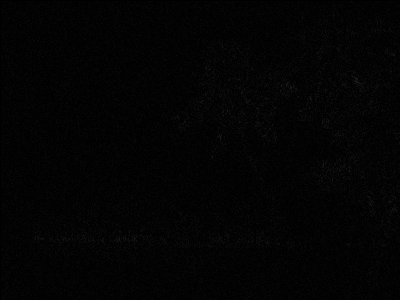
\includegraphics[scale=0.3]{output/p1-3-1-14}}
			}
			\label{fig:magnitudeinc50}
		}
		\quad
		\subfloat[Lowest 75\% pixels (\textbf{p1-3-1-15})]{
			{
				\setlength{\fboxsep}{1pt}
				\setlength{\fboxrule}{1pt}
				\fbox{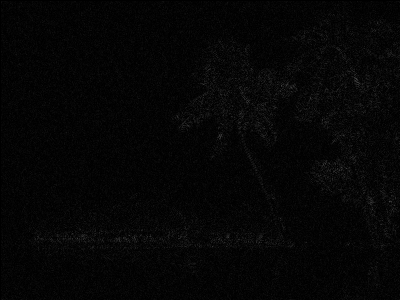
\includegraphics[scale=0.5]{output/p1-3-1-15}}
			}
			\label{fig:magnitudeinc75}
		}
		
		\caption{Results obtained by inverse Fourier transform using the lowest pixels on magnitude image.}
		\label{fig:magnitudeINC}
	\end{figure}
		
	Extracting the lowest pixels from magnitude is similar to use only low frequencies of the image, because of this the first row of Figure \ref{fig:magnitudeINC} is almost all black pixels. Proving our intuition looking at the magnitude brightness, as the original image has more high frequencies using low pixels does not describe a good portion of the image. \\
	
	However, we can see some of the contours being marked in Figure \ref{fig:magnitudeinc75}. This effect produces a image similar to the convolved image on Figure \ref{fig:conv}, which is a High-Pass-Filter. So, this process could be used as a high-pass filtering in the frequency domain. In contrast, The Figure \ref{fig:magnitudeDESC} show the same process using highest pixels on the magnitude image. \\
	
	\begin{figure}[!h]
		\centering
		\subfloat[Only highest pixel (\textbf{p1-3-1-17})]{
			{
				\setlength{\fboxsep}{1pt}
				\setlength{\fboxrule}{1pt}
				\fbox{
\includegraphics[scale=0.5]{output/p1-3-1-17}}
			}
			\label{fig:magnitudedesc1}
		}
		\quad
		\subfloat[Highest 25\% pixels (\textbf{p1-3-1-18})]{
			{
				\setlength{\fboxsep}{1pt}
				\setlength{\fboxrule}{1pt}
				\fbox{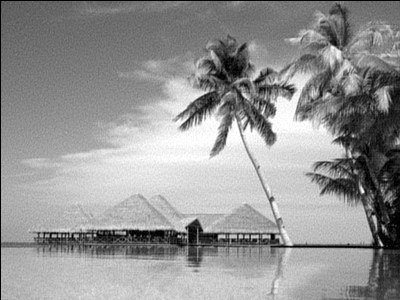
\includegraphics[scale=0.5]{output/p1-3-1-18}}
			}
			\label{fig:magnitudedesc25}
		}
		\quad
		\subfloat[Highest 50\% pixels (\textbf{p1-3-1-19})]{
			{
				\setlength{\fboxsep}{1pt}
				\setlength{\fboxrule}{1pt}
				\fbox{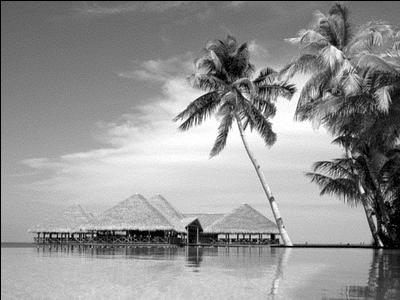
\includegraphics[scale=0.5]{output/p1-3-1-19}}
			}
			\label{fig:magnitudedesc50}
		}
		\quad
		\subfloat[Highest 75\% pixels (\textbf{p1-3-1-20})]{
			{
				\setlength{\fboxsep}{1pt}
				\setlength{\fboxrule}{1pt}
				\fbox{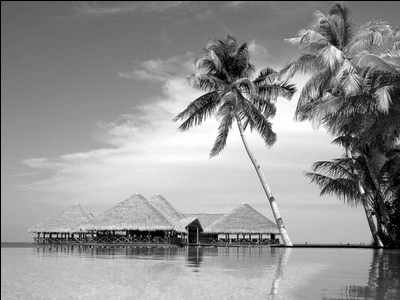
\includegraphics[scale=0.5]{output/p1-3-1-20}}
			}
			\label{fig:magnitudedesc75}
		}
		
		\caption{Results obtained by inverse Fourier transform using the highest pixels on magnitude image.}
		\label{fig:magnitudeDESC}
	\end{figure}
	
	As we would expect, even with less pixels from magnitude (25\%) the image was better represented, which indicates that a small part of the highest pixels on magnitude have most part of the information about the original image.  We can note that the quality of the reconstructed image is proportional with the percentage used on the magnitude image. The first image (Figure \ref{fig:magnitudedesc1}) does not have enough information to reconstruct the image, but the color already informs the predominant color intensity on original image (with just the highest pixel). \\
	
\end{itemize}

\newpage

In order to show that our implementation could also deal with colored images, we used the same experiment as before with a colored image. The Figure \ref{fig:magnitudeDESCColored} shows the result of using the highest values on the magnitude image on this colored image. \\


\begin{figure}[!h]
	\centering
	\subfloat[Only highest pixel (\textbf{p1-3-1-22})]{
		{
			\setlength{\fboxsep}{1pt}
			\setlength{\fboxrule}{1pt}
			\fbox{
\includegraphics[scale=0.5]{output/p1-3-1-22}}
		}
		\label{fig:magnitudedesc1}
	}
	\quad
	\subfloat[Highest 25\% pixels (\textbf{p1-3-1-23})]{
		{
			\setlength{\fboxsep}{1pt}
			\setlength{\fboxrule}{1pt}
			\fbox{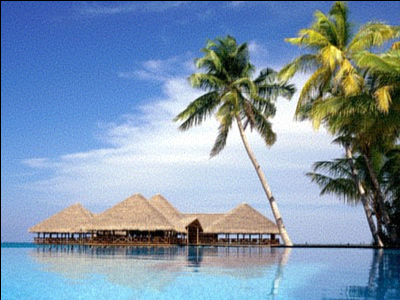
\includegraphics[scale=0.5]{output/p1-3-1-23}}
		}
		\label{fig:magnitudedesc25}
	}
	\quad
	\subfloat[Highest 50\% pixels (\textbf{p1-3-1-24})]{
		{
			\setlength{\fboxsep}{1pt}
			\setlength{\fboxrule}{1pt}
			\fbox{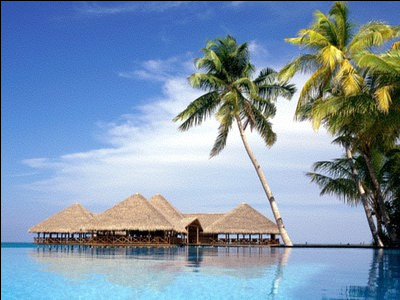
\includegraphics[scale=0.5]{output/p1-3-1-24}}
		}
		\label{fig:magnitudedesc50}
	}
	\quad
	\subfloat[Highest 75\% pixels (\textbf{p1-3-1-25})]{
		{
			\setlength{\fboxsep}{1pt}
			\setlength{\fboxrule}{1pt}
			\fbox{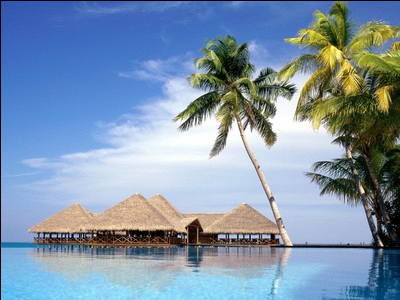
\includegraphics[scale=0.5]{output/p1-3-1-25}}
		}
		\label{fig:magnitudedesc75}
	}
	\quad
	\subfloat[Highest 100\% pixels (\textbf{p1-3-1-26})]{
		{
			\setlength{\fboxsep}{1pt}
			\setlength{\fboxrule}{1pt}
			\fbox{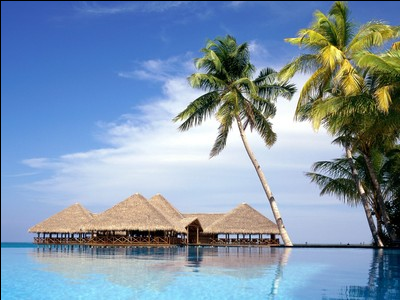
\includegraphics[scale=0.5]{output/p1-3-1-26}}
		}
		\label{fig:magnitudedesc100}
	}
	
	\caption{Results obtained by inverse Fourier transform using the highest pixels on magnitude image from the colored image.}
	\label{fig:magnitudeDESCColored}
\end{figure}

In order to use a colored image, the Fourier transform was applied in each color channel. Note that the Figure \ref{fig:magnitudedesc100} is the perfect reconstruction of the image \textbf{p1-1-0}, which indicates the process of Fourier transform was successful.

\newpage

\textbf{3.2 )} Blending \\

In order to obtain the blending on the frequency domain, we first transformed both images from spatial to frequency domain using the Fourier transform, which gives us the vectors magnitude and phase. Our first approach was to sum these vectors together, this approach obviously did not work, and the result can be seen in Figure \ref{fig:fourier1}. \\

\begin{figure}[!h]
	\centering
	{%
		\setlength{\fboxsep}{1pt}
		\setlength{\fboxrule}{1pt}
		\fbox{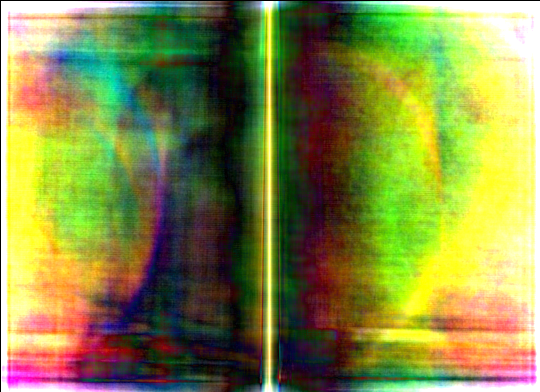
\includegraphics[scale=0.5]{report/Fourier.png}}
	}%
	\caption{Blending summing phase and magnitude vectors.}
	\label{fig:fourier1}
\end{figure}

After this approach, we have tried to implement the blending using different values for the phase and magnitude images, as example, we would use 50\% of highest values on both images and then perform the sum. At this time, we were expecting that the sum of the zeros (generated by the 50\% lowest values) could work with the summation. This approach did not work out, and the result is shown in Figure \ref{fig:fourier2}. \\

\begin{figure}[!h]
	\centering
	{%
		\setlength{\fboxsep}{1pt}%
		\setlength{\fboxrule}{1pt}%
		\fbox{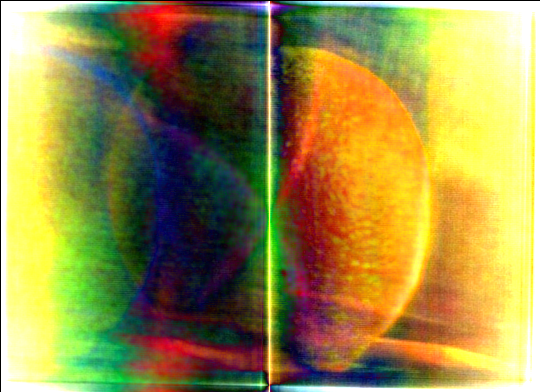
\includegraphics[scale=0.5]{report/Fourier50.png}}%
	}%
	\caption{Blending summing phase and magnitude vectors using the 50\% highest pixels from magnitude and phase images.}
	\label{fig:fourier2}
\end{figure}

After these tries, we started thinking about our results. Our conclusion was that no merging between the phase and magnitude would work as a blending. Moreover, we concluded that our approach was not working because of the way we were summing the vectors. We were dealing with complex numbers, and complex numbers do not add as normal numbers.  \\

So in order to fix this issue, we first construct a \emph{numpy} complex function $magnitude * np.exp(1j*phase)$. This way we could create one function to each image, and then sum them. Doing in this order \emph{numpy} knows that it is dealing with complex numbers, and it performs the right operation to sum te complex numbers. Which was what we were looking for, the result of this process is shown in Figure \ref{fig:blending}. \\

\begin{figure}[!h]
	\centering
	{%
		\setlength{\fboxsep}{1pt}%
		\setlength{\fboxrule}{1pt}%
		\fbox{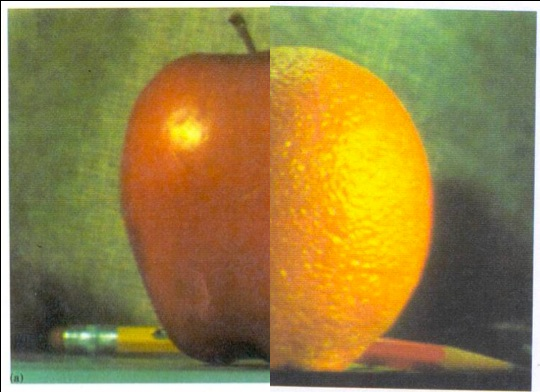
\includegraphics[scale=0.5]{output/p1-3-2-0.png}}%
	}%
	\caption{Blended image using \emph{numpy} complex sum.}
	\label{fig:fourier2}
\end{figure}

The generated image is a blend of two images, but when compared to the blending on spatial domain (Figure \ref{fig:aksda}) the results are not good. There is a high contrast between the images, we have tried some filtering approaches in order to solve it. However, none of the filtering ideas worked. \\

So, analyzing the result we figured that a pyramid could solve our problem (as it does on spatial domain). However, we had problems with the up-sampling and down-sampling. We could not change pixels arbitrary, mainly because one pixel on frequency domain represents more information on the original image, as seen in exercise \emph{\textbf{3.1} Exploring Fourier Space}. We did not have enough time to explore more this blending, but our intuition is that it might be possible to use pyramids with some ``trick'' applied to the frequency domain. 

\end{document}
